\chapter{NoSQL databáze}
Pojem NoSQL, poprvé použitý Carlem Strozzim v roce 1998 \cite{strozziNoSQL}, je obecný pojem zastřešující všechny databáze nepostavené na tradičním principu relačních SQL databází popsaného v předchozí kapitole. Zahrnuje tedy velké množství databázových serverů a technologií, které  vycházejí ze společné myšlenky.
Především je důležité zdůraznit, co NoSQL není – rozhodně to není NO SQL, tedy trendy odmítání relačních databází. Zkratka NoSQL znamená Not Only SQL, tedy uvědomění si toho, že relační databáze není jediná možnost řešení persistence dat. Že existují také alternativy, které mohou být v některých případech vhodnější. Zrod mnoha NoSQL databází je spjat s projekty známých internetových firem, které se musely vypořádat s obrovským množstvím dat – Facebook (Cassandra), Google (BigTable), Amazon (Dynamo), LinkedIn (Voldemort) atd. \cite{augiNoSQL}
O další rozdělení NoSQL databází se pokusilo už mnoho autorů, jako základní obecné kritérium pro další rozdělení je brán model ukládání dat.  Dále rozlišujeme tedy podle Ricka Cattella \cite{cattellStores} takto.

\begin{table}[h]
\centering
	\caption{Rozdělení NoSQL databázových serverů podle typu úložiště \cite{cattellStores}}
	\begin{tabular}{ |p{5cm}|p{5cm}| }
	\hline
	Typ NoSQL databáze & Databázové servery \\ \hline
	Key-Value Stores & Redis, Scalaris, Tokyo Tyrant, Voldemort, Riak, Memcached \\ \hline
	Document Stores & SimpleDB, CouchDB, \\
	& MongoDB, Terrastore \\ \hline
	Extensible Record Stores & BigTable, HBase, HyperTable, Cassandra \\ \hline
	Graph databases & Neo4j, FlockDB, \\ & AllegroGraph, GraphDB, \\ & InfiniteGraph \\ \hline
	Search Engines & ElasticSearch, Solr,\\ & Sphinx, Splunk \\ \hline
	\end{tabular}

	\label{tab:rozdeleniNoSQLServeru}
\end{table}
NoSQL databáze nebyly navrženy jako náhrada klasických SQL serverů, ale spíš si kladly za cíl vyřešit problémy, na něž současné SQL relační řešení nestačily. Některé typy webových aplikací totiž nevyžadují složité mechanismy ochrany dat, velké množství datových typů nebo transakční zpracování. Naopak vyžadují velmi rychlou odezvu a dostupnost. Proto první implementace NoSQL databází uměly pouze uložit nějakou hodnotu pod unikátním klíčem, sám databázový server nerozuměl hodnotám, které má uloženy a jen je "tupě"  vracel. Tyto NoSQL servery se používají i v dnešní době k ukládání velkých objemů jednoduchých dat (viz. \ref{section:keyValueDB}). Postupem času vzniklo několik skupin databázových serverů s rozdílnými vlastnostmi a způsobem uložení dat. Byly vytvořeny NoSQL databáze, podporující transakční zpracování. Vznikly také velmi zajímavé grafové databáze, které reprezentují relace mezi entitami pomocí hran grafu. Tyto databáze byly ale velmi koncepčně odlišné od klasických SQL databází, hlavně proto,že byly úzce přizpůsobeny pro řešení určitého problému a ani nebyly navrženy jako jejich náhrada. Řešením, které bylo navrženo jako alternativa k SQL serverům, byly \emph{dokumentově orientované NoSQL databáze} (viz. \ref{section:documentsDB}).
V těchto databázích se na entity pohlíží jako na dokumenty, které je možno shlukovat do pojmenovatelných množin (kolekcí) a pracovat s nimi velmi podobně jako s tabulkami SQL serveru.
Nejznámějším zástupcem dokumentově orientovaných databází je MongoDB, tutu databázi lze ve webové aplikaci použít ke stejnému účelu jako například MySQL.
\section{Výhody NoSQL databází}
Hlavní výhodou principu NoSQL databází je hlavně jejích jednoduchost a s tím spojená rychlost. Tato výhoda je ale zároveň i částečnou nevýhodou, jelikož se možnosti dotazování velmi omezily, je třeba složitější operace s daty provádět na straně aplikačního serveru vykonávacího obsluhu databáze. 
Mezi další výhody patři velmi dobrá podpora horizontálního škálování, tedy běhu na více serverech zároveň. S tím spojená schopnost práce s velmi velkými objemy dat, schopnost jednoduché replikace a flexibilní datové modely (neexistují schémata pro strukturu vstupních dat). Často jsou z těchto důvodů nasazovány na tzv. BigData aplikace, tedy aplikace, které pracují s velmi velkou množinou dat a potřebují s nimi rychle a efektivně pracovat. V posledních několika letech se objevilo velké množství nových databázových serverů, které pokrývají celou řadu oblastí při vývoji informačního systému. Můžeme dokonce NoSQL databáze používat jako primární úložiště dat, úložiště MongoDB nabízí vlastní souborový systém GridFS, který ukládá binární data po částech na více databázových serverech, čímž je činní velmi rychle dostupná. \cite{mongoDocs}

\subsection{Schemaless design}
Jedním z největších rozdílů mezi NoSQL a SQL databázemi je fakt, že vkládaná data nemají žádné předem dané schéma, jak mají vypadat. Tento fakt umožňuje vývojářům flexibilněji pracovat s datovými modely. Entita uložená v NoSQL databázi může nabývat mnoha podob, většinou se jedná o nějakou formu objektu, reprezentujícího objekty reálného světa s libovolným množstvím dvojic klíč - hodnota. NoSQL databáze je tedy úložištěm XML, YAML, JSON nebo BSON objektů. Těmto objektům se často říká záznamy nebo dokumenty. Hodnotou takového dokumentu může být i pole, další objekt nebo dokonce pole objektů. Schopnost téměř nekonečného zanořování objektů je další velkou výhodou datového modelu NoSQL databází.

Existuje několik tzv. objektových notací, jenž popisují přechod od objektu k řetězci. Tento proces se nazývá \emph{serializace dat}. Často používanou notací v NoSQL databázích je JSON, tuto notaci používá i NoSQL databáze MongoDB, který je použita v této práci. Vnitřně ovšem MongoDB ukládá tzv. BSON dokumenty, což je ale pouze binární obdoba formátu JSON.
\begin{figure}[h]
\begin{centering}
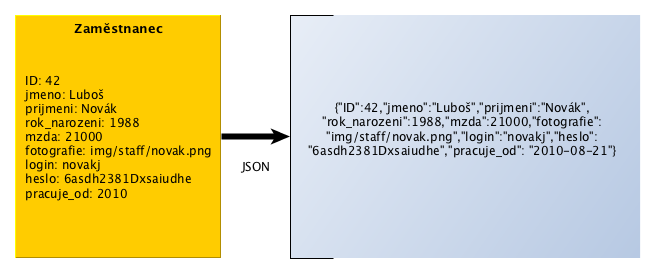
\includegraphics[scale=0.5]{obrazky/json-diagram} 
\caption{Ukázka konverze objektů notací JSON}
\end{centering}
\end{figure}

Pokud je potřeba v NoSQL databázích realizovat relaci mezi objekty, používají se identifikátory již existujících objektů jako prosté řetězcové hodnoty. Tento princip je velmi podobný mechanismu cizích klíčů ze světa SQL databází, NoSQL servery však tento mechanismem nedisponují. Databázový server tuto relaci nevidí a nemůže tedy kontrolovat její splnění, stejně tak získání obsahu odkazovaného objektu je nutné provést až v aplikaci.

\subsection{Sharding, distribuovaný návrh}
V době každý den narůstajících objemů dat, na Internetu uložených, je nutné s těmito daty rychle a účinně pracovat. Proto byly NoSQL databáze navrženy s ohledem na předpokládaný běh na více serverech. Díky tomu, že databáze běží ve více instancích, lze dobře rozdělovat zátěž, generovanou aplikací a jejími klienty. V současné době vzniká u některých aplikací také potřeba dynamicky upravovat výkon, vzhledem k vytížení aplikace jejími uživateli. Náhlé skokové nárůsty zátěže mohou nastat, ale díky distribuovanému návrhu většiny NoSQL databází, lze na tyto nárůsty dobře a rychle reagovat. Tato vlastnost moderních NoSQL databází se nazývá horizontální škálovatelnost a znamená zvýšení výkonu systému přidáním dalších serverů, nikoli zvýšením výkonu stávajících serverů (vertikální škálování). Dobrým příkladem jsou sportovní akce, které prakticky vždy zvýší požadavky na spojení s některými, často televizními, aplikacemi. Výkon databázového clusteru lze řidit i automaticky, existují nástroje, které v případě vysoké zátěže clusteru, automaticky vytvoří další virtuální servery.

Databáze MongoDB je od samého počátku jejího vývoje připravena k provozu v distribuovaném prostředí. K tomu tato databáze nabízí zajímavou funkcionalitu, tzv. \emph{sharding}. Jedná se o způsob rozdělení dat mezi servery zapojené v clusteru. Slovo shard, jak je v tomto případě nazýván jeden databázový server, lze do češtiny přeložit jako střep. Toto dělení obsahu databáze zmenšuje velikost dat, které musejí být uloženy na jednom serveru. Velikost uložených dat značně ovlivňuje rychlost zpracování požadavku nebo rychlost indexování databáze. Každý z těchto serverů obsahuje svojí část dat, která dohromady tvoří celou databázi. Je také možné definovat vlastní kritéria tohoto rozdělování, lze tedy například nová data ukládat na bližším serveru a ty starší mít uloženy jinde. Komunikaci v MongoDB clusteru řídí hlavní server, který také zajišťuje obsluhu požadavků na databázi \cite{mongoCluster}.

NoSQL databáze Redis není určena pro ukládání velkých objemů dat, a proto také neumožňuje ukládat svá data odděleně po částech mezi servery v clusteru. I přes to je Redis také často provozován v clusteru, jednotlivé servery tu zprostředkovávají čtení dat pro klienty, ukládání řídí hlavní databázový server. Redis cluster tedy využívá tzv. \emph{master-slave} architekturu  \cite{panykoNosql}.
\subsection{MapReduce a další agregační funkce}

Jednou z důležitých vlasností relačních SQL databází jsou agregace (shrnutí) dat. Jedná se o způsoby seskupování dat do celků podle zadaných kritérií. Většina NoSQL databází také disponuje bohatými agregačními možnostmi, plně podporující často používané způsoby agregace dat. Neznámější agregační funkcí je \emph{count}. Jejím úkolem je spočítat počet záznamů v databázi, které odpovídají dotazu. Dalšími často používanými agregačními funkcemi jsou funkce \emph{max} a \emph{min}, které slouží z zjištění maxima respektive minima. Lze také použít funkci \emph{group} pro prosté seskupení hodnot, podobné SQL příkazu \emph{GROUP BY}. Nebo je možné využít speciální agregační funkci zvanou \emph{MapReduce}. Tato funkce umožňuje programovat specializované agregace dat, většinou napsané v Javascriptu. Je tak možné získávat nová data nebo fakty ze stávající množiny dat. NoSQL databázové clustery dokonce tuto operaci distribuují mezi jednotlivé servery a zvyšují tím její výkon. Fungování tohoto principu popisuje následující schéma.

\begin{figure}[h]
\begin{centering}
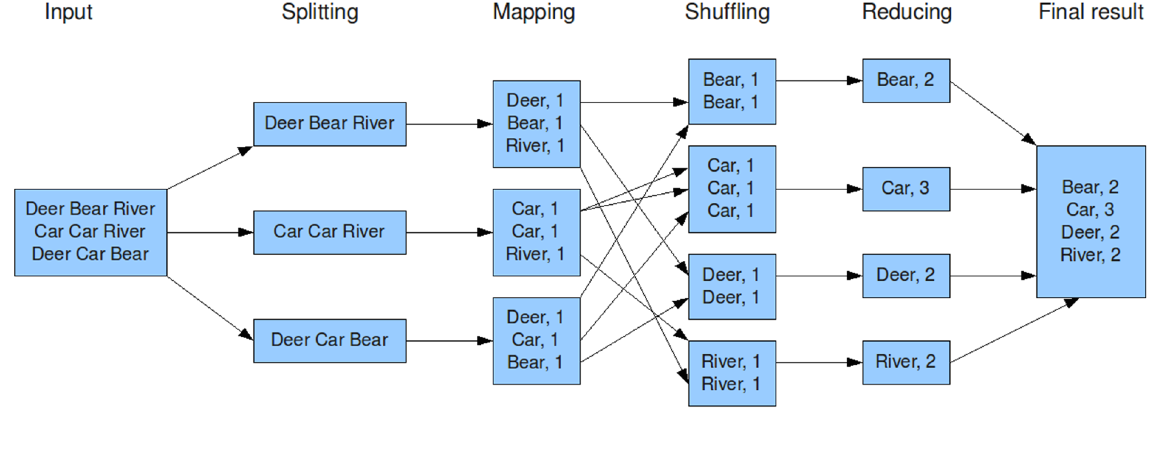
\includegraphics[scale=0.3]{obrazky/mapreduce}
\par\end{centering}
\caption{Ilustrace algoritmu MapReduce \cite{nosqlIrena}}
\end{figure} 
\FloatBarrier
\subsection{Master-Slave Replikace}
Většina z dnes používaných NoSQL databází nabízí nějakou formu zálohování dat. K výpadkům a haváriím vždy dochází a vysoká dostupnost jsou spolu s ochranou dat stěžejními předpoklady moderních NoSQL databází. Nejčastějším řešením tohoto problému je využití dvojic serverů, kde jeden slouží jako hlavní a druhý jako záložní. Úkolem hlavního serveru je zpracovávat požadavky na data a řídit samotnou databázi (mazání expirovaných dokumentů a další obslužné rutiny). Záložní server pouze drží kopii dat hlavního serveru, který se stará o její obnovování. Tento proces se nazývá \emph{master - slave replikace}, jednotlivé dvojice serverů potom většinou \emph{replica sety}. Tyto replica sety jsou popsány v praktické části, jsou totiž základní stavební jednotkou MongoDB databázového clusteru. 

Mechanismy zotavení databáze při výpadku hlavního serveru se mezi NoSQL databázemi značně liší. Dokumentově orientovaná databáze MongoDB používá mechanismus automatického přepnutí rolí serverů, tedy v případě pádu hlavního serveru převezme jeho úlohu server záložní, který se v tu chvíli stává hlavním. Připojíme-li ale původně hlavní databázový server zpět, stane se sám záložním serverem \cite{peteraMongo}. Podobný mechanismus používá i NoSQL databáze Redis, ta však například umožňuje připojit k slave serveru ještě další slave servery, pro které potom původní slave server vystupuje jako master. Problémem vícenásobné replikace je fakt, že operace zápisu je nutné vždy provádět na nejvýše postaveném serveru. Ostatní servery mohou uspokojovat požadavky klientů na data \cite{panykoNosql}. Tyto databáze se nazývají tzv. eventuálně konzistentní (Redis, MongoDB apod.), protože slave servery určené jen pro čtení se vždy nenachází v konzistentním stavu.

\begin{figure}[h]
\begin{centering}
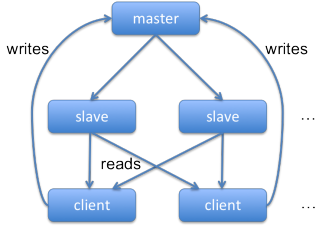
\includegraphics[scale=1.5]{obrazky/master-slave}
\par\end{centering}
\caption{Ukázka eventuální konzistence a komunikace mezi Master a Slave servery v MongoDB \cite{mongoConsist}}
\end{figure}
\pagebreak
\section{CAP teorém}
V roce 2000 na konferenci PODC představil Eric Brewer tři požadavky na distribuovaný systém, které údajně nemůžou být současně splněny. Definoval tři vlastnosti webové aplikace, které jsou bezpochyby žádoucí a od moderní aplikace očekávatelné, ale cíle těchto požadavků se navzájem vylučují \cite{gilbertCap}. Pro tento problém se vžil název \emph{Cap teorém}.

Tento teorém se skládá ze tři částí: Consistency (Konzistence), Availibility (Dostupnost) a Partition tolerance (Tolerance k rozdělení) \cite{cap}.

\vspace{0.25cm}
\noindent Gilbert a Lynch jako první definovali tyto části takto: \cite{gilbertCap}
\begin{itemize}
\item Konzistence (Atomická data) - V každém okamžiku jsou na všech uzlech distribuovaného systému stejná data
\item Dostupnost - Každý připojený klient bude obsloužen, i když chybovou hláškou.
\item Partition tolerance - Tento pojem znamená odolnost vůči výpadkům části distribuovaného systému.
\end{itemize}
Brewer ve své práci uvedl že všechny tři požadavky CAP teorému nelze nikdy splnit na 100\%  \cite{cap}. Z ilustrace teorému \ref{fig:cap} je dobře patrné, že nelze navrhnout databázový systém, který by zcela uspokojil všechny tři jeho požadavky. Další věcí, která je na schématu patrná, jsou tři skupiny databází, splňující alespoň dva požadavky teorému. Zástupce skupiny AP (\emph{Dostupnost a tolerance k rozdělení}) NoSQL databáze Dynamo klade důraz na to, aby každý připojený klient dostal odpověď na svůj dotaz a to i v případě výpadku napájení. U databáze HBase, patřící do skupiny CP (\emph{Konzistence dat a tolerance k rozdělení}), je zase hlavní konzistence dat \cite{panykoNosql}. Tradiční relační databázové systémy se označují jako CA (Konzistence a Dostupnost). 

Moderní NoSQL řešení se většinou vzdávají silné konzistence, aby získaly vyšší dostupnost. Tyto databáze pak nazýváme jako \emph{eventuálně konzistentní} \cite{peteraMongo}. Do této skupiny patří i databáze MongoDB, kterou se hlouběji zabývá tato práce \cite{mongoConsist}.

\vspace{0.5cm}
\noindent\emph{Jednotlivé skupiny databázových systémů, které splňují alespoň dvě části teorému.}
\begin{itemize}
\item AP (Availibility + Partitioning) - Dynamo, Voldemort, Cassandra
\item CP (Consistency + Partitioning) - MongoDB, Redis, HBase
\item CA (Consistency + Availibility) - MySQL, MSSQL, 
\end{itemize}

\begin{figure}[h]
\begin{centering}
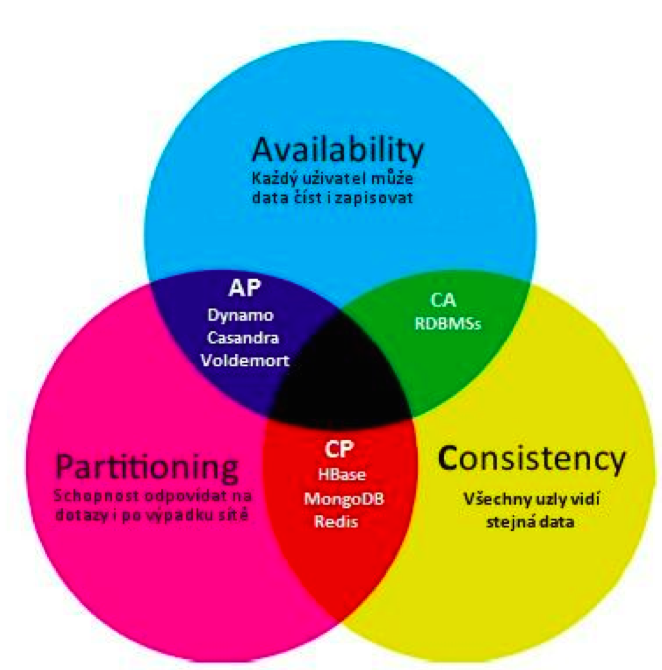
\includegraphics[scale=0.3]{obrazky/cap}
\par\end{centering}
\caption{Ilustrace CAP teorému \cite{panykoNosql}\label{fig:cap}}
\end{figure}

\section{BASE}
BASE byl navrhnut jako standard pro moderní ukládání velkých objemů dat v distribuovaných systémech. Je přímou reakcí na standard ACID u relačních databází. Tento princip za cenu omezení konzistence dat, zvyšuje jejich dostupnost. Christof Strach ho popisuje takto:\cite{strauchNosql}
\begin{itemize}
\item Basically Available - Systém stále běží, mohou nastat jen částečné chyby, nezpůsobující pád systému
\item Soft State - Systém je pružný, změny mohou nastávat (a nastávají) neustále
\item Eventual Consistency - Očekávání konzistentního stavu v budoucnu
\end{itemize}

\vspace{0.25cm}
\FloatBarrier
\begin{table}[h]
\caption{Srovnání ACID vs. Base \cite{nosqlSlides}}
\noindent\begin{tabular}{p{6.5cm} p{6.5cm}}
ACID (SQL) & BASE (NoSQL)\\ \hline
silná konzistence & slabá konzistence (stará data) \\
izolovanost & dostupnost na prvním místě \\
orientace na commit & přibližné odpovědi jsou OK \\
vnořené transakce & jednodušší, rychlejší \\
nezaručená dostupnost & dodávka dat "jak to jen půjde" \\
konzervativní (pesimistické) & agresivní (optimistické) \\
složitá evoluce kvůli schématu & jednoduchá evoluce (schemaless) \\
\end{tabular}

\end{table}
Případné nekonzistence jsou řešeny při čtení (verzování nebo nevalidní cache), při zápisu (distribuce změn) nebo asynchronně při replikaci dat \cite{nosqlSlides}.
\section{Typy NoSQL databází}
NoSQL databázový server je typicky jednoduché úložiště typu klíč -> hodnota, kdy hodnotou může být cokoliv (nejčastěji strukturovaný objektový zápis např. JSON) a klíč bývá unikátní identifikátor vygenerovaný samotnou databází. Toto je jedna z největších výhod těchto řešení, neomezuje totiž programátory žádnými modely předepisujícími strukturu vkládané entity. Typickým zástupcem takto jednoduché databáze je například Redis. 

Rozšiřujícím prvkem nad těmito úložišti může být další logické rozdělení uložených hodnot. Toto poskytují například dokumentově orientované databáze (např. MongoDB), kde každá vložená entita je uložena do nějaké kolekce, popisující typ a zařazení této entity. Díky návrhu podobnému SQL (kolekce vs. tabulky), jsou dokumentově orientované databáze použitelné jako přímá náhrada relačního SQL řešení.

Kvůli potřebám velmi rychlé správy propojených dat, vznikly také grafové databáze, které ukládájí dat a jejich vazby pomocí grafových struktur.

\subsection{Key-value úložiště}
\label{section:keyValueDB}
Prvním a také nejstarším typem NoSQL databází jsou key-value úložiště. Impulsem pro jejich vznik byla potřeba velmi rychle ukládat jednoduchá data s krátkou dobou uchování, často jen unikátní řetězce sloužící k nějaké formě identifikace.
Key-value databáze obecně je úložiště, kde každá uložená entita je indexována jen a pouze svým klíčem, nejčastěji nějakým unikátním identifikátorem ve formě řetězce. 
Vnitrně bývá implementováno jako jednoduchá hash tabulka \footnote{Datové struktura, sloužící k ukládání dvojic klíč-hodnota. Hashovací tabulka kombinuje výhody vyhledávání pomocí indexu a procházení seznamu.} nebo mapa \cite{beltrameKeyValue}.  

\vspace{0.5cm}
\noindent Tyto úložiště většinou poskytují jen tři nejzákladnější operace ke svojí obsluze a to:
\begin{itemize}
\item Uložení entity pod nějakým klíčem, ten je buď definován ve vstupních datech nebo vygenerován databázovým serverem
\item Získání entity podle klíče
\item Smazání entity podle klíče
\end{itemize}
Typů entit existuje velké množství, které je závislé na dané implementaci databáze. Key-value databáze Redis například nabízí řetězce, seznamy, mapy nebo množiny. Do těchto datových typů lze ukládat jednoduché řetězce i složité objekty \cite{redisDocs}.
Tato jednoduchost návrhu přináší velmi vysokou rychlost zpracování dat a jednoduchou škálovatelnost, je ale nutné veškeré složitější operace s daty provádět na aplikačním serveru. Databáze tedy skutečně zůstává jen tenkou vrstvou k uložení dat, která jsou však velmi rychle dostupná, díky možnosti běhu databáze na různém počtu strojů podle aktuální potřeby. Většina implementací key-value databází si drží svá data přímo v paměti, tato data jsou díky tomu ještě rychleji dostupná.
Důležitou vlastností key-value databází je možnost nastavení doby expirace uložených záznamů. Po uplynutí této doby se záznam v databázi automaticky smaže. Tato vlastnost je často využívána při ukládání uživatelských sezení, kdy expirace záznamu v databázi znamená odhlášení uživatele z aplikace z důvodu dlouhodobější nečinnosti \cite{redisDocs}.

Někteří zástupci těchto databází v omezené míře podporují transakční zpracování. Redis umožňuje řadit příkazy do fronty a pak je provést všechny najednou. V tomto případě databáze garantuje že příkazy uvnitř fronty budou provedeny najednou a žádný jiný požadavek nemůže být vyřízen, dokud se celá transakce nedokončí. Příkazy v transakci se provedou buď všechny úspěšně nebo dojde k jejímu selhání. Zde můžeme nalézt analogii se světem SQL databází, ale na rozdíl o SQL serverů, Redis nepodporuje žádný mechanismus, který by se dal přirovnat k příkazu \emph{ROLLBACK}, známým z SQL transakcí. Databáze tedy neposkytuje žádnou možnost reagovat na selhání transakce. Redis také disponuje možností master-slave replikace, která probíhá asynchronně, což umožňuje pracovat s databází i v průběhu replikace. Pro zajištění velmi vysoké dostupnosti databáze, je vyvíjen nástroj Redis Sentinel, umožňující automatickou správu Redis clusteru. Tento nástroj umožňuje monitorování běžících instancí Redisu, jejich obsluhu a automaticky přepíná mezi dvojicemi replikovaných serverů, pokud dojde k výpadku některého z nich \cite{redisDocs}.

Tyto databáze zajišťují ukládání dat pro specifickou oblast webové aplikace, pro kterou jsou výborně optimalizovány, například slouží jako úložiště uživatelských sezení nebo kešovaných dat. Kvůli jejich úzké specializaci není ve většině případů absence plnohodnotných transakcí problém. 
Mezi nejznámější key-value úložiště patří vedle již zmíněného Redisu, také Riak, Dymamo, Voldemort, Berkeley DB, HamsterDB nebo Memcached. 
Do této kategorie patří také Cassandra, jedna z prvních NoSQL databází vyvinutá ve společnosti Facebook \cite{cassandra}.

Většina key-value databází včetně Redisu je volně dostupná. Redis je dokonce distribuován pod licencí BSD, je ho tedy možná zdarma používat i na komerčních projektech \cite{redisDocs}.

\begin{figure}[h]
\begin{centering}
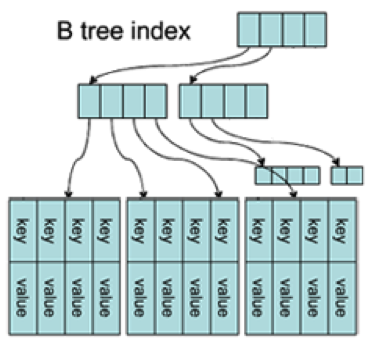
\includegraphics[scale=1]{obrazky/keyvaluedb-strom}
\par\end{centering}
\caption{Ukázka uložení dat v key-value databázích \cite{tolitStorelist} \label{fig:keyValueTree}}
\end{figure}

\subsection{Dokumentově orientované databáze}
\label{section:documentsDB}
Dokumentově orientované databáze představují evoluci NoSQL databází, nabízejí kompromis mezi přílišnou jednoduchostí a dostatečnou rychlostí zpracování. Jejich  nejznámější zástupce, MongoDB, je dlouhodobě nejpoužívanější NoSQL databázi nasazovanou do ostrého provozu  \cite{enginesRanking}.
MongoDB je také jednou ze dvou databází, kterou se hlouběji zabývá tato práce. Tato databáze byla vyvinuta společnost 10gen v roce 2007, jako součást své platform-as-a-service platformy. V roce 2009 tato společnost vydala první open source verzi své databáze. Název této NoSQL databáze je odvozen od anglického slova "humongous", které popisuje něco velmi velkého nebo chcete-li obrovského.  Stabilní verze, připravená pro produkční nasazení, vyšla v roce 2010. MongoDB je napsáno v jazyce C++. Tato databáze byla od začátku navržena pro běh v clusteru, jedná se proto o jednu z jejich klíčových vlastností  \cite{peteraMongo}.

Základním prvkem pro ukládání dat je zde dokument, kterým je míněn objekt (entita) s jedinečným identifikátorem a množinou párů klíč-hodnota, jež mohou být do sebe dále libovolně vnořovány. Na rozdíl od systémů typu klíč-hodnota většinou umožňují také sekundární indexování atributů \footnote{Možnost přidání indexu na kterýkoliv klíč entity.},  a co do funkcionality jsou robustnější. Pro ukládání dat užívají JSON, XML nebo podobné strukturované formáty  \cite{regnerVse}.
Dalším důležitým prvkem je kolekce, která popisuje a obaluje dokumenty, v ní uložené. Vnitřní rozdělení dokumentů do kolekcí doplňuje logické uspořádání entit do celků, podle nichž lze dokumenty opět získávat. Pro získání všech dokumentů určitého typu, už tedy není potřeba žádná složitější aplikační logika, stačí jen získat celou kolekci.

Kolekce v MognoDB fyzicky obsahuje libovolný počet BSON \footnote{Binární podoba formátu JSON.} dokumentů, jehož maximální možná velikost je 16MB. Větší dokumenty lze ukládat pomocí souborového systému GridFS, který rozdělí dokument a několik částí (chunků) a ty poté obsluhuje jako jeden dokument. Dotazovacím jazykem databáze MongoDB je Javascript. V tomto jazyce lze také psát vlastní uložené procedury \cite{mongoDocs}. 

Kvůli tomu je tato databáze velmi oblíbená především u vývojářů moderních javascriptových SPA\footnote{Single Page Application - jednostránková webová aplikace, napsaná kompletně v klientském Javascriptu.} a mezi vývojáři v NodeJS. Databáze MongoDB je distrubována pod licencí GNU AGPL v3.0 pro serverovou část a Apache 2 Licence pro klientskou část, je tedy možné ji používat zdarma i pro komerční využití.

\begin{lstlisting}[caption=Příklad databázového dotazu v MongoDB]
db.zamestnanci.find(
    {
       prijmeni: 'Novak',
       mzda: {'$gte':10000}
    }
);
\end{lstlisting}
\noindent Tento dotaz vyhledá v kolekci \emph{zamestnanci} všechny zaměstnance kteří je jmenují Novák a mají mzdu větší než 10000 Kč.
Funkce \emph{find()} slouží k získávání dat z kolekce pomocí definovaných omezení. Je ekvivalentem příkazu SELECT u SQL databází. První parametrem funkce je tzv. \emph{matcher}, který udává podmínky, jenž musí splňovat entita v kolekci. V našem případě musí obsahovat příjmení Novák. Konstrukce \$gte je z anglického "\emph{greater than equals}" a znamená matematickou operaci větší nebo rovno. Funkce \emph{find()} umožňuje používat i druhý parametr, tzv. projekci. Ta umožňuje definovat strukturu vrácených dokumentů, projekce tedy funguje naprosto stejně jako výčet sloupců v SQL příkazu SELECT \cite{mongoDocs}.
\pagebreak

\begin{lstlisting}[caption=Odpověď MongoDB databázového serveru]
{
   jmeno: 'Pavel',
   pozice: 'Manager',
   prijmeni: 'Novák'
   mzda: 15800,
   oceneni: [
   	{nazev: 'Nejlepší Manažer 2014', udeleno: 2014-07-08}
   	],
   umisteni: 'management',
   fotografie: 'images/staff/pnovak.png',
   prava: ['user','manager'],
   ve_spolecnosti: 2001
}

{
   jmeno: 'Jiří'
   prijmeni: 'Novák',
   pozice: 'Accountant',
   umisteni: 'ekonomicke',
   mzda: 11200,
   ve_spolecnosti: 2010
}
{
   jmeno: 'Jakub'
   prijmeni: 'Novák',
   pozice: 'Developer',
   umisteni: 'developers',
   mzda: 37000,
   prava: ['user','developer'],
   ve_spolecnosti: 2005
}
\end{lstlisting}

Kolekci není potřeba nijak vytvářet, je vytvořena automaticky při vložení prvního záznamu. Přepínání mezi databázemi probíhá analogicky s SQL světem pomocí příkazu \emph{USE}. Data se vkládají pomocí příkazu \emph{insert}, jejímž jediným parametrem je dokument ve formátu JSON, který bude uložen do zvolené kolekce. Kolekce, nad níž provádíme operace, se v MongoDB uvádí jako objekt, nad kterým voláme funkce \emph{find} nebo \emph{insert} \cite{mongoDocs}.

\pagebreak
\begin{lstlisting}[caption=Vložení dokumentu do databáze test a kolekce zamestnanci v MongoDB]
use test;
db.zamestnanci.insert(
	{
		jmeno: 'Jakub',
		prijmeni: 'Josef',
		pozice : 'CEO',
		umisteni: 'management',
		mzda: 250000,
		fotografie: 'images/hq/jjosef.png',
		prava: ['user', 'manager', 'hq', 'admin'],
		ve_spolecnosti: 2000 	
	}
);
\end{lstlisting}

Unikátní identifikátor záznamu (v SQL světě známý jako primární klíč) v MongoDB nalezneme pod klíčem \emph{\_id}. Pokud není \_id specifikováno ve vkládaném dokumentu (jako v ukázce výše), bude automaticky vytvořeno databází. Databáze MongoDB generuje 12 bytový řetězec, který se skládá z náhodného čísla, data vytvoření dokumentu a jedinečného identifikátoru stroje a procesu  \cite{mongoDocs}.

Kolekce v MongoDB lze také omezit maximálním počtem záznamů (tzv. Capped Collections), tyto kolekce se výborně hodí pro ukládání dat, které je třeba uchovávat pouze po omezenou dobu, například nějaké souhrny nebo logy. Ukládání dat do kolekce lze omezit také časově. Samotné dokumenty v MongoDB také umožňují expiraci (odstranění) dokumentu po určitém čase. Tomuto parametru se říká TTL\footnote{Time to live.} a v MongoDB se nastavuje jako index \cite{mongoDocs}.

\begin{lstlisting}[caption=Vytvoření indexu s parametrem expirace TTL 3600 sekund]
db.log_events.ensureIndex( { "createdAt": 1 }, { expireAfterSeconds: 3600 } )
\end{lstlisting}

Pro pokročilejší získávání dat lze v MongoDB používat i tzv. matchery, kterými lze definovat kritéria, podle nichž lze výběr omezit. Matchery vždy začínají znakem \$ a nabízejí bohaté možnosti dotazování, řeší chybějící operátory v dotazech a jsou přímým NoSQL ekvivalentem příkazu WHERE ze světa SQL databází. Samotný MongoDB matcher je klasický objekt, na jehož klíči je název matcheru (operátor) a hodnotou je hodnota, která bude argumentem operátoru. Jednotlivé matchery lze shlukovat pomocí logických operátorů \emph{\$and},  \emph{\$or} a \emph{\$not} \cite{mongoDocs}.
\pagebreak

\noindent\emph{Nejčastěji používané matchery v MongoDB}
\begin{itemize}
\item \$gt - hodnota prvku je větší než, ekvivalent znaku >
\item \$gte - hodnota prvku je větší nebo rovno, ekvivalent znaku >=
\item \$lt - hodnota prvku je menší než, ekvivalent znaku <
\item \$lte - hodnota prvku je menší nebo rovno, ekvivalent znaku <=
\item \$ne - hodnota prvku je se nerovná, ekvivalent znaku !=
\item \$nin - prvek neexistuje
\item \$exists - existuje klíč
\item \$type - klíč je specifického typu
\item \$mod - operace modulo, ekvivalent znaku %
\item \$regex - dotazování pomocí regulárního výrazu
\item \$text - provede fulltextové vyhledávání
\item \$where - hodnota prvku bude porovnána pomocí Javascriptové funkce
\item \$all - hodnotou prvku je pole a obsahuje všechny zadané prvky
\item \$elemMatch - hodnotou prvku je pole a prvním elementem pole je zadaný element.
\end{itemize}

Matcherů v MongoDB existuje celá řada a pokrývají veškeré běžné matematické operace. Existují také matchery poskytující výpočet tzv. Haversinovské vzdálenosti, tedy vzdálenosti mezi dvěma body v prostoru, zadanými pouze GPS souřadnicemi. K tomu slouží geometrické matchery \emph{\$near} a \emph{\$nearSphere} \cite{mongoDocs}.

\begin{lstlisting}[caption=Ukázka složitějšího dotazu na MongoDB databázi]
db.zamestnanci.find(
   {
     umisteni: 'management',
     prava: 'hq',
     $or: [ { mzda: { $gt: 15000, $lte: 100000} }, { ve_spolecnosti: { $lt: 2010 } } ]
   }
)
\end{lstlisting}

Tento dotaz získá všechny zaměstnance, kteří jsou umístění v sekci management a mají buď mzdu větší než 15000 Kč a menší než 100 000 Kč, nebo jsou ve společnosti déle než 4 roky (v roce 2014). Jinak řečeno, jejich rok nástupu je nižší než 2010. Ačkoliv se na klíči \emph{prava} nachází pole, v dotazu je použit jen prostý řetězec. V tomto případě totiž databáze pole otestuje na existenci tohoto řetězce \cite{mongoDocs}.

Další důležitou vlastností každé databáze je možnost řazení, v SQL prováděné pomocí klauzule \emph{ORDER BY}. MongoDB nabízí metodu \emph{sort()}, která přijímá objekt s klíčem podle kterého bude seřazení probíhat a číslem udávajícím směr tohoto řazení. Směr se v MongoDB udává pomocí dvou čísel, \emph{1} znamená vzestupně a je ekvivalentem SQL klauzule \emph{ASC}. Sestupné řazení (DESC) se v MongoDB udává jako \emph{-1}. Omezení velikosti výsledku je v MongoDB dostupné pomocí jasně použitelné funkce \emph{limit()} příjímající počet dokumentů, které budou vráceny. \cite{mongoDocs}. 

\begin{lstlisting}[caption={Ukázka sestupného řazení podle mzdy a omezení v MongoDB}]
db.zamestnanci.find(...).sort({ mzda: -1}).limit(20)
\end{lstlisting}
Možnosti dotazování jsou v dokumentově orientované databázi MongoDB skutečně bohaté a dalo by se  říci, že dokonce převyšují obvyklé možnosti SQL serverů. Databáze je dostupná pro Linux, Windows, Mac OS X a Solaris.

Dalšími zástupci dokumentově orientovaných databází jsou CouchDB,  RavenDB nebo RethinkDB.
CouchDB je databází, která vychází z dokumentově orientovaného projektu Lotus Notes. Její hlavní vývojář Damien Katz na tomto produktu dlouho pracoval u společnosti IBM. Tato databáze se koncepčně velmi podobná MongoDB, avšak nepoužívá kolekce, ale přináší například pohledy na data nebo replikaci na klientská zařízení. Komunikace s ní probíhá, na rozdíl od MongoDB, pomocí vestavěného REST API. Administrační úkony v databázi je tedy nutné provádět například pomocí nástroje cURL \footnote{Nástroj příkazové řádky usnadňující odesílání HTTP požadavků.} \cite{strauchNosql}.
\subsection{Sloupcově orientované databáze}
Sloupcově orientované databázové systémy vycházejí z projektu Google BigTable  \cite{changBigtable}. Jsou opět určeny především vysokozátěžovým systémům a jsou vysoce optimalizovány pro paralelní zpracování dotazů. Můžeme si je představit jako klasickou tabulku. Každý záznam (řádek) zde má svůj unikátní identifikátor, ovšem fyzicky se data ukládají nikoliv po řádcích, jak je běžné u relačních databází, nýbrž po sloupcích. Je tak rychlejší například vyhledat záznamy s určitou hodnotou atributu a zároveň se šetří diskový prostor serveru, jelikož nemusí být vyhrazeno žádné místo navíc pro prázdné buňky \cite{regnerVse}.
Tyto databáze se hodí pro použití v datacentrech, pro CRM systémy\footnote{Customer Relationship Management - Systémy pro řízení vztahů se zákazníky.}, knihovny nebo podobná nasazení. Sloupcově orientované databáze se obecně hodí pro správu velkého množství stejných nebo podobných dat, které ukládají na disk po sloupcích zvlášť. To umožňuje při čtení načíst přesně tolik atributů (sloupců), kolik je zrovna potřeba, a tím šetřit prostředky databázového serveru \cite{columnDB}. 

Následující obrázek \ref{fig:columnDB} dobře ilustruje odlišnosti ve struktuře dat sloupcově orientovaných databází. Pokud aplikace potřebuje nová data a žádá o obsah atributů \emph{saleid} a \emph{date}, databázový server skutečně získá jen tyto sloupce a vrátí jejich obsah. Naopak pokud aplikace často získává celé objekty, nebo provádí agregační funkce, není pro ni sloupcově orientovaná databáze příliš vhodná.

\begin{figure}[h]
\begin{centering}
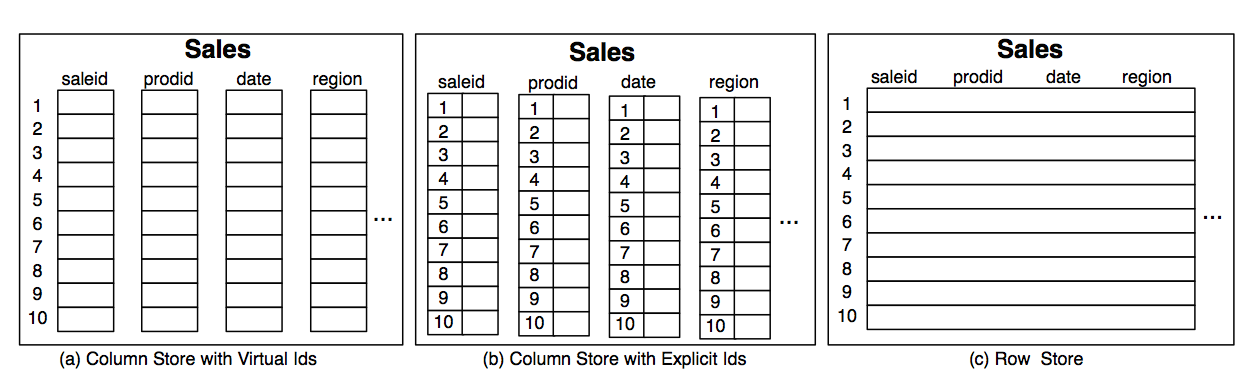
\includegraphics[scale=0.3]{obrazky/column-vs-row}
\par\end{centering}
\caption{Porovnání sloupcově orientované databáze s relační databází založenou na řádcích. \label{fig:columnDB} \cite{columnDB}}
\end{figure}
Mezi nejznámější sloupcově orientované databáze patří MonetDB, HBase, BigTable nebo HyperTable.

\subsection{Grafově orientované databáze}
Grafově orientované databáze představují specifický typ databázových systémů založený na grafech. Tyto databáze se hodí pro reprezentaci sítí a jejich typologii, jako jsou například sítě počítačové, dopravní nebo sociální. Používají se tedy k práci s daty, která mají mezi sebou velké množství vazeb. Do databáze se ukládají uzly s určitými vlastnostmi a také hrany mezi těmito uzly \cite{graphDb}.

Hlavním přínosem je schopnost rychle vyhledávat příslušné uzly i ve velmi rozsáhlém grafu. Grafové databáze totiž při vyhledávaní používají pokročilé grafové algoritmy, které jsou pro dané použití mnohem rychlejší a efektivnější než by byla běžná relační databáze \cite{graphDb}.  

Grafová databáze se obecně skládá ze dvou základních prvků, vrcholů (nodes) a hran (edges). Každý z těchto vrcholů obsahuje několik hran vedoucích k dalším vrcholům. Tyto hrany reprezentují vazby. Hrany mezi vrcholy mají vždy označen směr, víme tedy, ze kterého vrcholu vstupuje a ze kterého vystupuje. Mohou však existovat i vrcholy, které na sobě žádné hrany nemají \cite{graphDb}. 

Samotná data jsou nejčastěji uložena ve vrcholech, ačkoli grafová databáze Neo4j nabízí možnost ukládání dat i v hranách \cite{neo4j}.
Pravděpodobně nejznámější grafovou databází je Neo4j. Tato databáze, která je postavena na programovacím jazyku Java, je velmi oblíbená pro ukládání hustě propojených dat a je k tomuto účelu v poslední době i často nasazována. Na rozdíl o většiny NoSQL databází, databáze Neo4j podporuje ACID transakce. Ty ale drží v paměti, což může být u větších grafů problém. Je proto doporučeno velké transakce dělit na několik menších, pokud nehrozí porušení konzistence dat v databázi. \cite{neo4j}.

Komunikace s Neo4j serverem probíhá přes vestavěné REST API, které nabízí rozhraní dostupné pro vývojáře jakéhokoliv jazyka. Hlavním komunikačním formátem je JSON \cite{neo4j}.

\begin{figure}[h]
\begin{centering}
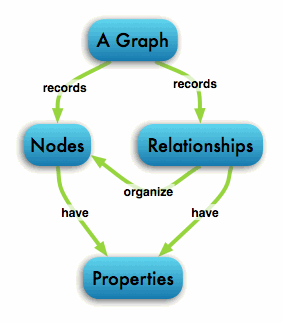
\includegraphics[scale=0.5]{obrazky/neo4j-graph}
\par\end{centering}
\caption{Vztahy mezi entitami v Neo4j. \cite{neo4j}}
\end{figure}

\FloatBarrier
Grafová databáze Neo4j používá speciální dotazovácí jazyk Cypher, pomocí něj je možné vytvářet, získávat, nebo editovat data v databázi. Základem syntaxe tohoto jazyka je vzor, dotazování na data probíhá pomocí mechanismu známého jako \emph{pattern matching} \footnote{Způsob porovnávaní sekvence znaků proti zadanému vzoru.}. Data se tedy získávájí pomocí porovnávání zadaných vzorů a struktury grafu. Samotný vzor se skládá z jednoho nebo více uzlů s jejich vzájemnými vztahy, štítky a vlastnostmi. Vlastnost v Neo4j reprezentuje dvojice klíč - hodnota, která je již v této práci dobře popsána. Druhou důležitou částí jazyka Cypher jsou tzv. klauzule. Klauzule jako takové jsou dobře známým pojmem z SQL databází a jejich syntaxe a použití v Neo4j jsou velmi podobné. Základ jazyka tvojí klauzule \emph{MATCH}, která umožňuje hledání podle zadaného vzoru. Klauzule WHERE slouží k zadání podmínek dotazu, naprosto analogicky jako u SQL databází \cite{cypher}. 
 
\begin{lstlisting}[caption={Ukázka Neo4j dotazu, který získá uživatele s ID 123}]
MATCH (user:User)
WHERE user.Id = 1234
RETURN user
\end{lstlisting}

Modifikace uložených dat funguje podle očekávání prostřednictvím příkazu \emph{SET} \cite{cypher}.
\begin{lstlisting}[caption={Ukázka Neo4j dotazu který provede změnu věku uživatele 123}]
MATCH (user:User)
WHERE user.Id = 123
SET user.Age = 25
\end{lstlisting}

Další klauzule \emph{CREATE, MATCH, SET, REMOVE a DELETE} slouží pro manipulace s daty. V rámci dotazování je také možné používat speciální grafové funkce jako například \emph{shortestPath} pro nalezení nejkratší cesty v grafu, nebo \emph{allPaths} pro nalezení všech přípustných cest \cite{cypher}.
\begin{lstlisting}[caption={Ukázka Neo4j dotazu, který vytvoří nového uživatele,  poté ho spojí s uživatelem 123, který ho pozval (role invitee)}]
MATCH (invitee:User)
WHERE invitee.Id = 123
CREATE invitee-[:INVITED]->(invited:User {newUser})
\end{lstlisting}

Neo4j server je dostupný pro Linux, Mac OS X a Windows ve 4 základních verzích licencovaných podle jejích použití. Základní verze \emph{Neo4j Comunity} je určena pro open source projekty a je distribuována zcela zdarma. Tato verze obsahuje různá omezení, je například ochuzena o monitorovací nástroje nebo clustering. Druhou variantou je verze \emph{Neo4j Personal}, která nabízí plnou verzi databáze zcela zdarma. Tato varianta je ale přípustná pouze pro malé firmy do příjmu 100 tisíc dolarů a maximálně 3 zaměstnanců. Třetí možnost licencování, určená především pro startupy, se jmenuje \emph{Neo4j Startups}. Je k dispozici firmám s ročním příjmem nižším než 5 milionů dolarů a v případě startupů s počáteční investicí nižší než 10 milionů dolarů. Cena této licence je 12 tisíc dolarů (asi 250 tisíc Kč) za kalendářní rok. Ostatním společnostem, které nesplňuji výše uvedená kritéria je cena licence stanovena individuálně \cite{neo4jLicence}.

Další zajímavou grafovou databázi představuje AllegroGraph. Jedná se o zástupce tzv. RDF databází. RDF objekt, v ní uložený, je takzvaný triplet ve tvaru subjekt-predikát-objekt a představuje datový model reality. Můžeme si ho představit jako orientovaný ohodnocený graf, kde hrana začíná v subjektu, je ohodnocena predikátem a končí v objektu. Subjekt představuje datový zdroj, většinou URI. Predikátem se chápe nějaká vlastnost nebo aspekt daného subjektu, vyjadřuje tedy jeho vztah k danému objektu. Tento objekt tvoří hodnotu a může obsahovat čísla nebo řetězce. Častěji je ale objektem URI dalšího subjektu a vznikne tím zřetězení. Tímto způsobem lze velmi dobře popisovat například rodinné vztahy nebo lze nad RDF grafem také dokazovat fakta. Dotazování na RDF databáze většinou realizuje dotazovací jazyk SPARQL \cite{nosqlSlides}.

\subsection{Vyhledávací enginy}
Zvláštní skupinou serverů, které se vlastně také dají považovat za NoSQL databáze, jsou vyhledávací enginy. Tyto databáze jsou vysoce optimalizovány pro rychlé prohledávání velkého množství textových dat. Jejich úkolem je rozložit věty na jednotlivá slova a poté kořeny těchto slov spolu se informacemi o synonymech zaindexovat do vlastní databáze. Zároveň tento engine obsahuje vlastní sadu slov, které se nebudou indexovat, protože se jedná o běžné výrazové prostředky jazyka: jednoduchá slova, předložky nebo spojky. Poté je  možné se fulltextově dotazovat na objekty v ní uložené \cite{searching}.

Z již napsaného vyplývá, že tyto procesy zpracování textových dat je třeba konfigurovat přímo pro daný jazyk ve kterém bude engine používán \cite{searching}. Tyto databáze se využívají především pro účely fulltextového vyhledávání. Proprietární řešení od společností Google nebo Microsoft pravděpodobně používá podobné mechanismy zpracování textových dat.
\begin{figure}[h]
\begin{centering}
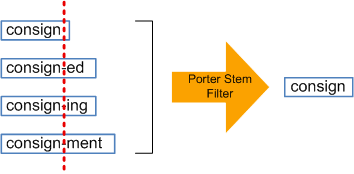
\includegraphics[scale=0.9]{obrazky/stemming}
\par\end{centering}
\caption{Ukázka stemmingu, tvorby kořene slov \cite{grailsLucene}}
\end{figure}

Nejznámějšími zástupci vyhledávacích enginů je Sphinx Search nebo ElasticSearch. Zejména  ElasticSearch se začíná v poslední době často používat pro fulltextové vyhledávání, momentálně je nejpoužívanější databází svého druhu \cite{enginesRanking}.


\section{Monitoring databáze}
Obecně asi každý počítačový server je dobré monitorovat, aby mohl jeho administrátor kontrolovat jeho stav a reagovat na případné problémy. U databázových serverů je důležitost monitoringu vysoká hlavně při použití distribuovaných řešení. Některé z NoSQL databázových serverů již v základu obsahují nějakou formu monitoringu, často tenký webový server zobrazující informace o databázi. Například MongoDB po svém spuštění spouští také webový server obsahující administrační rozhraní. Tento server běží na portu o 1000 vyšším než je nastavený port databáze. Tedy implicitně na portu 28017 \cite{mongoAdmin}. Vestavěné webové  administrační rozhraní obsahuje také grafová databáze Neo4j \cite{neo4jAdmin}. Existuje také velké množství aplikací pro monitoring NoSQL databázových serverů, namátkou lze zmínit například Redsmin pro správu Redis databáze, nebo OpsCenter na monitoring a vizualizaci dat pro databázi Cassandra.

Následující dva obrázky představují ukázku vestavěného webového rozhraní v MongoDB.
Databáze je spuštěna na standartním portu 27017, webové rozhraní je tedy dostupné na portu 28017.
 
\begin{figure}[h]
\begin{centering}
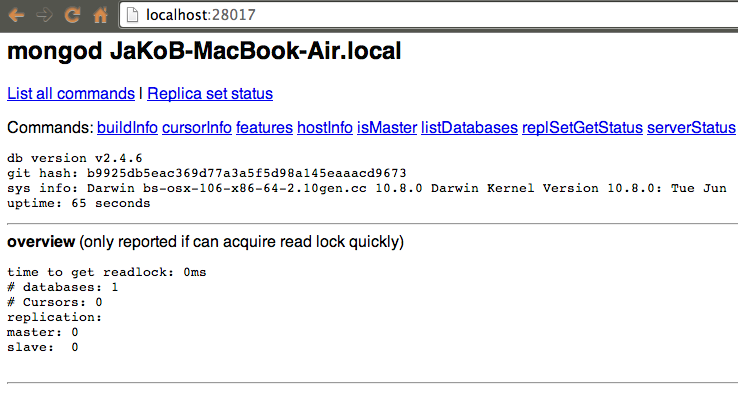
\includegraphics[scale=0.4]{obrazky/mongo-admin-top}
\par\end{centering}
\caption{Stav MongoDB serveru ve webovém rozhraní\label{fig:mongoAdmin}}
\end{figure}

\FloatBarrier
První z nich ilustruje stav serveru, jeho verzi a kód sestavení. Dozvíme se zde také info o systému a dobu běhu serveru. Na druhém obrázku vidíme připojené klienty k databázi. Skutečně připojení klienti vždy začínají slovem \emph{conn}, ostatní jsou systémové rutiny. Například rutina TTLMonitor se stará o mazání expirovaných (neplatných) záznamů \cite{mongoAdmin}.

\begin{figure}[h]
\begin{centering}
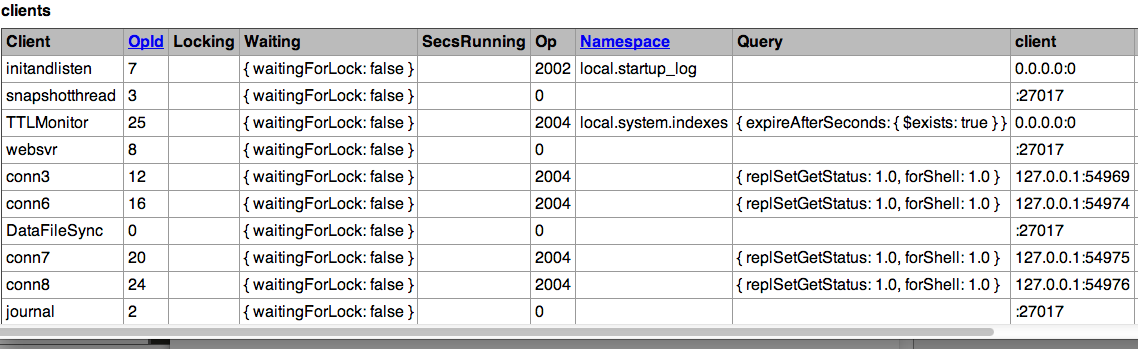
\includegraphics[scale=0.3]{obrazky/mongo-admin-clients}
\par\end{centering}
\caption{Seznam připojených klientů MongoDB serveru ve webového rozhraní\label{fig:mongoAdmin}}
\end{figure}

\FloatBarrier
Grafová databáze Neo4j také disponuje administračním rozhraním, pomocí kterého lze sledovat stav databázového serveru, nebo provádět manipulovce s daty. Toto rozhraní standardně běží na portu 7474  \cite{neo4j}.

\section{Rozhraní k programovacím jazykům}
Důležitou vlastností každé databáze je schopnost komunikace s aplikacemi. Existuje ale bohužel velké množství jazyků, ve nichž lze,  ať už webové nebo desktopové aplikace, psát. Komunikaci aplikací s databázemi zajišťují většinou tzv. ovladače. Některé databázové ovladače jsou součástí použitého jazyka, jiné je třeba přidat do prostředí, v němž je aplikace vyvíjena. Databázové ovladače jsou většinou volně dostupné na oficiálních stránkách nejznámějších programovacích jazyků.

Po připojení aplikace k databázi je proveden dotaz na nějaká data. Ovladač zprostředkuje získání dat a vrátí je aplikaci ve formátu vhodném pro daný jazyk (JSON objekt, PHP array, Python dict, Ruby hash apod.). Tyto ovladače je však nutné vytvořit zvlášť pro každý jazyk a databázi. 

Druhou možností, jak řešit komunikaci databáze s aplikací, je použití tzv. \emph{REST API}. Jedná se v podstatě o rozhraní webového serveru, který však na základě došlých HTTP požadavků vykonává obsluhu databáze. Velkou výhodou tohoto řešení se použití standardizovaného formátu komunikace, což při vývoji aplikace znamená možnost použití jakéhokoliv jazyka schopného používat protokol HTTP. Rozhraní typu REST je definováno jako HTTP server, které implementuje čtyři základní metody: \emph{GET, POST, DELETE a PUT.} Tyto čtyři metody pokrývají čtyři základní operace s daty známé jako CRUD \footnote{Create, Retrieve, Update, Delete.} \cite{rest}.

Velkou výhodou REST API je možnost jeho použití v Javascriptových aplikacích, které běží v prohlížeči uživatele. Vzhledem k rozmachu těchto aplikací na dnešním Internetu, jsou REST API stále žádanější funkcionalitou a je pravděpodobné, že ho brzy některá z NoSQL databází doplní.

Dnes REST API nabízí například dokumentově orientovaná databáze CouchDB, vyhledávací engine Elasticsearch nebo grafová databáze Neo4j.

\section{Bezpečnost}
Při práci s SQL serverem je běžná existence velkého množství uživatelů a skupin s různými úrovněmi pravomocí. SQL servery obvykle obsahují propracovaný bezpečnostní subsystém, je možné definovat různá oprávnění (čtení, zápis, změna struktury apod.) na úrovni tabulky nebo celé databáze. 

Naproti tomu NoSQL databáze většinou ve výchozím nastavení vůbec žádnou autentizaci nevyžadují. Je to proto, že pro účely testování nebo provozu malé aplikace stačí nechat databázi dostupnou pouze lokálně, tím pádem s ní může komunikovat jen aplikace běžící na stejném serveru. Toto řešení je potencionálně nebezpečné, protože při průniku na server se útočník dostane bez větších problémů i k databázi. Na druhou stranu, přímé napadení serveru je na tolik závažnou zranitelností, že i zabezpečený databázový server může být napaden nebo vymazán.  

Ale i NoSQL databáze nabízejí bohaté možnosti autorizace, přihlášení k databázi je většinou dostupné přes příkaz \emph{AUTH} (Redis, MongoDB) a vyžaduje klasickou dvojici přihlašovacího jména a hesla. Například v MongoDB se uživatele definují pro každou databázi zvlášť pomocí speciální kolekce \emph{users}. Ukládat uživatele standardně pomocí prostředků databáze jako kterákoliv jiná data je standardním postupem v oblasti NoSQL databází, což vede například k tomu, že na key-value databázi Redis lze kvůli jejímu návrhu velmi rychle paralelně útočit hrubou silou \cite{redisBF}.

Také komunikace aplikace s databázovým serverem většinou probíhá nešifrovaně, hrozí tedy riziko MITM \footnote{Men In The Middle.} útoků. Jedná se o útok, kde útočník stojí mezi serverem a klientem a odchytává nebo mění jejich komunikaci \cite{mitm}. Toto riziko hrozí například u databáze MongoDB, která má ve výchozím stavu zcela vypnutou autentizaci a existuje v něm také \emph{admin} databáze, ze které je možné pracovat se všemi databázemi na serveru. Velmi dobrou bezpečnostní politikou je přiřadit k MongoDB serveru IP adresu, na které běží aplikace a všechny ostatní požadavky ignorovat. Dobrou radou je také nepoužívat výchozí port \cite{mongoHacking}.

\section{Možnosti škálování v NoSQL databázích}
Jednou z hlavních výhod NoSQL databází je výborná podpora pro horizontální škálování, tedy zvyšování výkonu databáze zvyšováním počtu serverů zapojených do databázového clusteru. Většina NoSQL databází přímo poskytuje vestavěné nástroje pro provoz na více serverech, plně distribuovatelný návrh byl totiž jedním z hlavních důvodů jejich vzniku. Centralizovaná SQL řešení totiž v některých velmi datově náročných aplikacích přestávala stačit. Problémem ovšem není ani tak obrovská velikost dat v databázi uložených, ale spíše velký objem klientů, kteří chtějí s databází pracovat najednou a pokud možno s minimálními časy odezvy. Proto nejznámější webovou aplikací, která už dlouho používá NoSQL řešení, je americká sociální síť Twitter. 

Databázový cluster se obvykle skládá z velkého počtu dvojic datových serverů, které se mezi sebou replikují. Tento koncept se nazývá Master - Slave replikace a je dobře známý i ze světa SQL databází. Každý z těchto datových serverů má uloženu pouze část dat celé databáze. Tyto datové servery zpravidla vůbec neumožňují čtení dat, které probíhá z hlavního serveru (často označován jako router). Tento server má za úkol předávat získaná data aplikaci pomocí databázového rozhraní. Router zjistí, na kterém serveru se požadovaná data nachází, a vrátí je. Informace o fyzickém uložení dat na jednotlivých serverech buď uchovává přímo router nebo jsou získávány z konfiguračních serverů. Konfigurační servery slouží ke správě dat, vědí kde se která data nachází a současně řídí i jejich ukládání. Tento koncept používá například dokumentově orientovaná databáze MongoDB. Tato práce v praktické části představí principy fungování a konfiguraci MongoDB clusteru. 

\section{Srovnání MongoDB s MySQL}
V následující kapitole je provedeno teoretické srovnání databází MySQL a MongoDB, které se navzájem překrývají v svých případech užití, je proto vhodné je porovnat. Databáze budou porovnávány z několika hlavních hledisek, důležitých pro rozhodnutí vývojáře, kterou z těchto databází ve své aplikaci použije. Srovnání výkonu následuje v praktické části této práce.

\vspace{0.25cm}
\noindent Tato tabulka dobře ilustruje rozdílné koncepty v obou databázích.
\begin{table}[h]
\centering
	\caption{Porovnání terminologie MySQL vs. MongoDB \cite{mongoMySQLMapChart}}
    \begin{tabular}{ |p{7cm}|p{7cm}| }
    \hline
    \multicolumn{2}{|c|}{Terminologie} \\ \hline
    MySQL & MongoDB \\ \hline
	databáze & databáze \\	
	tabulka & kolekce \\
	řádek & dokument \\
	sloupec & pole \\
	index & index \\
	relace mezi tabulkami & embedded dokumenty a linkování \\ \hline
    \end{tabular}
    \label{tab:porovnaniTerminologie}
\end{table}

\FloatBarrier
\subsection{Návrh}
Rozdíl v návrhu těchto databází je značný, je v něm patrné stáří technologie MySQL, která nepočítala s distribuovanou formou fungování. Naproti tomu MongoDB vzniklo v roce 2007 a bylo vytvořeno pro dnes známý Internet. MySQL je také na rozdíl od MongoDB zástupcem silně konzistentních serverů. Data v MySQL tedy musejí mít přesně danou podobu. Obě databáze mají potencionální cíl využití webovou aplikaci, která potřebuje ukládat strukturovaná data: uživatele, články, komentáře, fotografie a jiná data. Klasickou cestou MySQL vývojáře by bylo vytvořit pro každou entitu aplikace databázovou tabulku, navrhnout její atributy a relace na jiné tabulky. Také každá změna v aplikaci by poté musela být reflektována i ve struktuře databáze. 

MongoDB dává vývojářům větší volnost v ukládání dat, je možné ukládat jakékoliv objekty, přidávat atributy dokumentů, nové kolekce nebo celé databáze. Díky teoreticky nekonečné možnosti zanořování MongoDB dokumentů, lze některé vazby řešit přímo na úrovni dokumentu, jak ilustruje obrázek níže. Tato databáze vývojářům ale neposkytuje žádné záruky, jak bude požadovaný objekt vypadat. Pokud je třeba ověřovat jeho strukturu, je nutné to provést až v aplikaci \cite{mongoDocs}.

\begin{figure}[h]
\begin{centering}
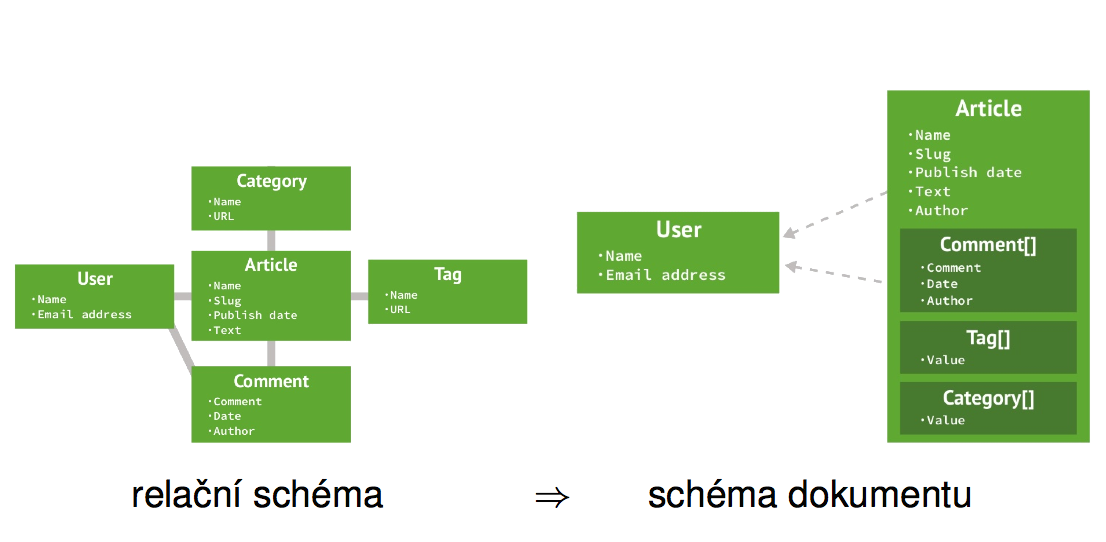
\includegraphics[scale=0.3]{obrazky/schema-vs-documents}
\par\end{centering}
\caption{Srovnání způsobu ukládání dat v MySQL a MongoDB databázích. \cite{nosqlSlides}}
\end{figure}

\subsection{Syntaxe}
Relační databáze MySQL používá dotazovací jazyk SQL, zatímco MongoDB dotazuje pomocí volání javascriptových metod. Rozdíl v syntaxi dotazů je velký, ale u NoSQL databáze MongoDB je možné vidět snahu o přiblížení se terminologii SQL serverů. Následující tabulka dobře ilustruje srovnání syntaxe databází MySQL a MongoDB.
\begin{table}[h]
\centering
    \caption{Porovnání syntaxe základních operací MongoDB vs. MySQL \cite{mongoMySQLMapChart}}
    \begin{tabular}{ |p{1.9cm}|l|l| }
    \hline
    \multicolumn{3}{|c|}{Srovnání syntaxe MySQL a MongoDB} \\ \hline
    Operace & MySQL & MongoDB \\ \hline
	Vytvoření tabulky & 
	\begin{lstlisting}
CREATE TABLE users (
 id int(11) NOT NULL 
 	AUTO_INCREMENT,
 user_id varchar(30),
 age int(11),
 status char(1),
 PRIMARY KEY (id)
)
 \end{lstlisting}
 & 
 \begin{lstlisting}
db.users.insert( {
  user\id: "abc123",
  age: 55,
  status: "A"
} ) 
 \end{lstlisting} 
 \\ \hline
	Přidání atributu &
	\begin{lstlisting}
ALTER TABLE users
ADD join_date DATETIME
	\end{lstlisting} &
	\begin{lstlisting}
db.users.update(
 { },
 {$set: {date:new Date()}},
 { multi: true })	
	\end{lstlisting}	
	 \\ \hline
	 Odstranění atributu &
	\begin{lstlisting}
ALTER TABLE users
DROP COLUMNT join_date 
	\end{lstlisting} &
	\begin{lstlisting}
db.users.update(
    { },
    { $unset:{join_date:""}},
    { multi: true })	
	\end{lstlisting}	
	 \\ \hline
	Vytvoření indexu &
	\begin{lstlisting}
CREATE INDEX
 idx_user_asc_age_desc ON
 users(user_id, age DESC)
	\end{lstlisting}
	&
	\begin{lstlisting}
db.users.ensureIndex( 
{ user_id: 1, age: -1 } )
	\end{lstlisting}
	\\ \hline
	Vložení dat &
	\begin{lstlisting}
INSERT INTO 
users(user_id, age, status)
VALUES ("bcd001",
        45,
        "A")	
	\end{lstlisting} &
	\begin{lstlisting}
db.users.insert(
   { 
   user_id: "bcd001",
   age: 45,
   status: "A" }
)
	\end{lstlisting} \\ \hline
	Získání dat &
	\begin{lstlisting}
SELECT user_id, status
FROM users
WHERE status = "A"	
	\end{lstlisting}
	&
	\begin{lstlisting}
db.users.find(
    { status: "A" },
    { user_id: 1,
      status: 1,
      _id: 0 })
	\end{lstlisting}
	\\ \hline
	Editace dat &
	\begin{lstlisting}
UPDATE users
SET status = "C"
WHERE age > 25	
	\end{lstlisting} &
	\begin{lstlisting}
db.users.update(
   { age: { $gt: 25 } },
   { $set: { status: "C" } },
   { multi: true }
)	
	\end{lstlisting} \\ \hline
	Odstranění dat &
	\begin{lstlisting}
DELETE FROM users
WHERE status = "D"	
	\end{lstlisting}
	&
	\begin{lstlisting}
db.users.remove({status:"D"})
	\end{lstlisting} 
	\\ \hline
    \end{tabular}
    \label{tab:porovnaniSyntaxe}
\end{table}

\FloatBarrier
\subsection{Podpora platforem}
MySQL je databáze vyvíjená v C++ a je dostupná na všech běžně používaných systémech včetně FreeBSD. MongoDB je vyvíjeno ve stejném jazyce a je dostupné pro Windows, Linux, Mac OS X a Solaris.

Databázové ovladače jsou dostupné pro všechny nejpoužívanější jazyky, PHP podporuje práci s MySQL nativně, podporu MongoDB je nutno doplnit rozšiřujícím modulem. Moduly pro MongoDB jsou dostupné pro .NET platformu, Javu, Ruby, Python, Perl a další jazyky.

\subsection{Možnosti migrace existujících aplikací}
I když se MongoDB prezentuje jako vhodná náhrada MySQL řešení, rozdíly v návrhu těchto dvou databází jsou tak velké,  že případná migrace již provozované aplikace by znamenala velké změny v jejím kódu. Pokud aplikace používá nějaký ORM \footnote{Object Relation Mapping - automatické mapování databázových tabulek do objektů jazyka aplikace.} framework, možnosti migrace se díky další abstraktní vrstvě zvyšují. Oblíbený ORM framework Doctrine totiž nabízí databázový ovladač i pro MongoDB. Tyto frameworky, které mapují objekty aplikace na dokumenty v MongoDB, se nazývají ODM - Object Document Mapping frameworky. Obecně lze ale říci, že MongoDB je dobrou volbou spíše pro nové aplikace, migrovat již provozovanou aplikaci se příliš nevyplatí. Jedinou situací, kdy by byla migrace nezbytná, je pokrytí opravdu velké zátěže na kterou už relační databázové řešení nestačí. V tuto chvíli pomůže distribuované řešení na bázi MongoDB.

\subsection{Nástroje}
Pro relační databázi MySQL existuje celá řada nástrojů včetně oficiální desktopové aplikace MySQL Workbench. Častěji se ale pro správu databáze používají webová rozhraní. Nejznámější z nich, phpMyAdmin je vyvíjen již od roku 1998 \cite{phpMyAdmin}. Mezi jeho alternativy patří SQLBuddy nebo Adminer. Nástrojů pro MongoDB rozhodně neexistuje takové množství jako pro MySQL, vzhledem k tomu jak nová technologie MongoDB je. 

Utility pro import a export dat databáze jsou součástí distribuce MongoDB serveru. Také existuje několik desktopových aplikací pro správu této databáze. Velmi kvalitní aplikací je MongoDB Management Service, která zprostředkovává správu databáze v cloudu, včetně nasazování databázových serverů a tvorby záloh. Nástroj UMongo,  sloužící také pro správu clusteru, je dostupný pro Linux, Windows i Mac OS X.  Mezi aplikace určené především k práci s daty, patří Mac OS X klient MongoHub nebo komerční řešení MongoVUE postavené na platformě .NET. Existuje i několik webových rozhraní, podporující MongoDB. Jedním z nich je i již zmiňovaný Adminer. Zajímavým nástrojem je také aplikace Edda, která slouží k vizualizaci logů z MongoDB databáze. Přehledné shrnutí nástrojů pro MongoDB lze nalézt na webu \emph{mongodb-tools.com}.

\subsection{Licencování}
Databáze MongoDB je dostupná pod licencí GNU AGPL v3.0, je tedy zdarma pro komerční i nekomerční účely. Mongo klient je distribuován pod licencí Apache.

Zdarma pro veškeré účely je i MySQL, distribuované pod licencí GPL. MySQL navíc nabízí i placenou komerční alternativu, kterou je ale nutné použít, pouze ve specifických případech použití, například pokud chceme MySQL server dodávat jako součást naší aplikace \cite{payMysql}.